\documentclass{article}

\usepackage[utf8]{inputenc}
% \usepackage{braket}
\usepackage{enumitem}
\usepackage{multirow}
\usepackage{xcolor}
\usepackage[T1]{fontenc}
% \usepackage[french]{babel}
\usepackage{amssymb}
\usepackage{mathtools}
\usepackage{ntheorem}
\usepackage{amsmath}
\usepackage{amssymb}
\usepackage[ a4paper, hmargin={2cm, 2cm}, vmargin={3cm, 3cm}]{geometry}
\usepackage{hyperref}
\usepackage{capt-of}

\usepackage[braket, qm]{qcircuit}
\usepackage{graphicx}

\usepackage{tikz}
\usetikzlibrary{angles,quotes}

\theoremstyle{plain}
\theorembodyfont{\normalfont}
\theoremseparator{~--}
\newtheorem{exo}{Exercise}%[section]

\newcommand{\norm}[1]{\left\lVert#1\right\rVert}

\usepackage{hyperref}
\hypersetup{
    colorlinks,
    citecolor=black,
    filecolor=black,
    linkcolor=blue,
    urlcolor=blue
}

\usepackage{xcolor}

\definecolor{codegreen}{rgb}{0,0.6,0}
\definecolor{codegray}{rgb}{0.5,0.5,0.5}
\definecolor{codepurple}{rgb}{0.58,0,0.82}

\usepackage{listings}
\lstdefinestyle{mystyle}{
    commentstyle=\color{codegreen},
    keywordstyle=\color{magenta},
    numberstyle=\tiny\color{codegray},
    stringstyle=\color{codepurple},
    basicstyle=\ttfamily\footnotesize,
    breakatwhitespace=false,
    breaklines=true,
    captionpos=b,
    keepspaces=true,
    numbers=left,
    numbersep=5pt,
    showspaces=false,
    showstringspaces=false,
    showtabs=false,
    tabsize=2
}
\lstset{style=mystyle}

\title{TP QPE and Shor}
\author{Valeran MAYTIE}
\date{}

\begin{document}
  \maketitle

  \section{Small Practice}

    \begin{figure}[!htb]
      \begin{center}
      \scalebox{1.5}{
        \Qcircuit @C=1.0em @R=0.2em @!R { \\
            \nghost{{q}_{0} :  } & \lstick{{q}_{0} :  } & \gate{\mathrm{H}} & \ctrl{1} & \ctrl{2} & \qw & \meter & \qw & \qw & \qw\\
            \nghost{{q}_{1} :  } & \lstick{{q}_{1} :  } & \qw & \targ & \qw & \meter & \qw & \qw & \qw & \qw\\
            \nghost{{q}_{2} :  } & \lstick{{q}_{2} :  } & \qw & \qw & \targ & \qw & \qw & \meter & \qw & \qw\\
            \nghost{\mathrm{{c} :  }} & \lstick{\mathrm{{c} :  }} & \lstick{/_{_{3}}} \cw & \cw & \cw & \dstick{_{_{\hspace{0.0em}1}}} \cw \ar @{<=} [-2,0] & \dstick{_{_{\hspace{0.0em}0}}} \cw \ar @{<=} [-3,0] & \dstick{_{_{\hspace{0.0em}2}}} \cw \ar @{<=} [-1,0] & \cw & \cw\\
        \\ }}
    \end{center}
    \caption{Circuit that calculate $\frac1{\sqrt2}(|000\rangle+|111\rangle)$}
    \label{fig:cir1}
    \end{figure}

    To compute $\frac1{\sqrt2}(|000\rangle+|111\rangle)$, we created the
    circuit shown in Figure \ref{fig:cir1}. Firstly we apply an Hadamard Gate on
    the first qubit to have a 50/50 chance of having it at 1 or 0.
    If it's equal to one then with a \textit{CNot} gate controlled by the first
    qubit we inverse $q_1$ and $q_2$, so they are all equal to 1.
    Else nothing change and it remains at 0.

    When you run it, you'll find the right measurements the result is
    roughly 50/50, 000 or 111.

    The code for this exercise is shown in Listing \ref{lst:pra}

\begin{lstlisting}[language=Python, label= lst:pra,
                   caption=Code that generates the circuit in Figure \ref{fig:cir1}]
q = QuantumRegister(3)
c = ClassicalRegister(3)
qc = QuantumCircuit(q,c)

qc.h(q[0])

qc.cnot(q[0],q[1])
qc.cnot(q[0],q[2])

qc.measure(q, c)\end{lstlisting}

  \newpage
  \section{QPE}

    We construct the operator $\mathbf{U}$ with this matrix :

    \[
      \begin{pmatrix}
        1 & 0 & 0 & 0 \\
        0 & 1 & 0 & 0 \\
        0 & 0 & 1 & 0 \\
        0 & 0 & 0 & e^{2i \pi \frac 6 8}
      \end{pmatrix}
    \]

    \subsection{Math Questions}

    \begin{enumerate}
      \item What is doing this operator ?
        (`2j` is in Python the complex number $2\cdot i$)

      The operator $\mathbf{U}$ compute this :
      \begin{itemize}
        \item $\mathbf{U} |00\rangle = |00\rangle$
        \item $\mathbf{U} |01\rangle = |01\rangle$
        \item $\mathbf{U} |10\rangle = |10\rangle$
        \item $\mathbf{U} |11\rangle = e^{2i \pi \frac 6 8}|11\rangle$
      \end{itemize}

      \item On how many qubits does it act ?

        This operator act on 2 qubits.

      \item What are its eigenvalues/eigenvectors ?

        \begin{center}
        \begin{tabular}{c c}
          eigenvectors & eigenvalues \\
          $|00\rangle$ & 1 \\
          $|01\rangle$ & 1 \\
          $|10\rangle$ & 1 \\
          $|11\rangle$ & $e^{2i \pi \frac 6 8}$
        \end{tabular}
        \end{center}

      \item For each eigenvector, what should QPE return with 3 bits of
        precisions, as seen in the course ?

        \begin{center}
        \begin{tabular}{c c}
          eigenvectors & QPE return \\
          $|00\rangle$ & 000 \\
          $|01\rangle$ & 000 \\
          $|10\rangle$ & 000 \\
          $|11\rangle$ & 110
        \end{tabular}
        \end{center}
    \end{enumerate}

  \newpage
  \subsection{Implementing QPE}

  \begin{figure}[!htb]
    \begin{center}
    \scalebox{1.0}{
      \Qcircuit @C=1.0em @R=0.2em @!R { \\
          \nghost{{eig}_{0} :  } & \lstick{{eig}_{0} :  } & \gate{\mathrm{H}} & \ctrl{3} & \qw & \qw & \multigate{2}{\mathrm{IQFT}}_<<<{0} & \meter & \qw & \qw & \qw & \qw\\
          \nghost{{eig}_{1} :  } & \lstick{{eig}_{1} :  } & \gate{\mathrm{H}} & \qw & \ctrl{2} & \qw & \ghost{\mathrm{IQFT}}_<<<{1} & \qw & \meter & \qw & \qw & \qw\\
          \nghost{{eig}_{2} :  } & \lstick{{eig}_{2} :  } & \gate{\mathrm{H}} & \qw & \qw & \ctrl{1} & \ghost{\mathrm{IQFT}}_<<<{2} & \qw & \qw & \meter & \qw & \qw\\
          \nghost{{phi}_{0} :  } & \lstick{{phi}_{0} :  } & \gate{\mathrm{X}} & \multigate{1}{\mathrm{unitary\string^1}}_<<<{0} & \multigate{1}{\mathrm{unitary\string^2}}_<<<{0} & \multigate{1}{\mathrm{unitary\string^4}}_<<<{0} & \qw & \qw & \qw & \qw & \qw & \qw\\
          \nghost{{phi}_{1} :  } & \lstick{{phi}_{1} :  } & \gate{\mathrm{X}} & \ghost{\mathrm{unitary\string^1}}_<<<{1} & \ghost{\mathrm{unitary\string^2}}_<<<{1} & \ghost{\mathrm{unitary\string^4}}_<<<{1} & \qw & \qw & \qw & \qw & \qw & \qw\\
          \nghost{\mathrm{{ceig} :  }} & \lstick{\mathrm{{ceig} :  }} & \lstick{/_{_{3}}} \cw & \cw & \cw & \cw & \cw & \dstick{_{_{\hspace{0.0em}0}}} \cw \ar @{<=} [-5,0] & \dstick{_{_{\hspace{0.0em}1}}} \cw \ar @{<=} [-4,0] & \dstick{_{_{\hspace{0.0em}2}}} \cw \ar @{<=} [-3,0] & \cw & \cw\\
      \\ }}
    \end{center}
    \caption{QPE circuit}\label{fig:qpe}
  \end{figure}

  \begin{lstlisting}[language=python, label=cpe_code,
                     caption=Code that generate the QPE circuit]
eig = QuantumRegister(size_eig, name="eig")
phi = QuantumRegister(size_phi, name="phi")
ceig = ClassicalRegister(size_eig, name="ceig")
qc = QuantumCircuit(eig,phi,ceig)

qc.x(phi[0])
qc.x(phi[1])
for i in range(0, size_eig):
    qc.h(eig[i])
    qc.append(U.power(2**i).control(), [eig[i], phi[0], phi[1]])

qc.append(QFT(size_eig).inverse(), eig)
qc.measure(eig, ceig)\end{lstlisting}

    \subsection{Exact result}

    \begin{enumerate}
      \item Is it the expected result ?

        Yes, we calculated $110 \equiv \frac 1 2 + \frac 1 4 = \frac 6 8$
        so $\mathbf U |11\rangle = e^{2i\pi \theta}|11\rangle$.

        With 3 bits precision $\theta$ is equal to $\frac 6 8$
        seen in Exercise 2.1.1.

      \item Change the $\frac68$ of the phase of $U$: use $\frac18$,
        then $\frac28$... Is QPE returning the correct answer ?

        Yes, we have $001$, $010$, $\ldots$ and $111$, when we tested up to
        $\frac 7 8$, because there is enough precision. But then we get the
        right result modulo 8.

      \item Change the precision : use $4$ qubits for ``eig'', and change the
        fraction in the phase of $\mathbf{U}$ to $\frac{10}{16}$ : is QPE indeed
        returning $10$ in binary ?

        We have 10 written in binary. It works because we have enough precision
        to get the real eigenvalues.

      \item Move to $5$ bits of precision is it still working ?

        It works, we have $\frac 1 2 + \frac 1 8 = \frac{10}{16}$

    \end{enumerate}

    \newpage
    \subsection{Approximate result}

      The QPE approach calculations with 3-bits precision are given in the
      table below

      \begin{center}
      \begin{tabular}{c | l }
        \multirow{2}*{value} & number of times \\
                             & obtained \\
        \hline
        000     & 21  \\
        001     & 34  \\
        010     & 178 \\
        011     & 708 \\
        100     & 39  \\
        101     & 20  \\
        110     & 10  \\
        111     & 14  \\
        \hline
        average / $2^3$ & 0.365
      \end{tabular}
      \end{center}

      We can see that the average divided by two power of precision is close to
      the eigenvalue ($\frac 1 3$). And the more you increase the accuracy,
      the closer you get to $\frac 1 3$.
    \subsection{Superposition}

    By changing the phi initialization to $\frac1{\sqrt2}(|\phi_1\rangle + |\phi_2\rangle)$
    Two calculations are performed in parallel, one to calculate the eigenvalue
    of eigenvectors $|11\rangle$ and $|00\rangle$.

    For the phase it works very well we have :

    \begin{center}
      \begin{tabular}{c | c | l}
        \textit{phi} & \textit{eig} & \\
        \hline
        00 & 000 & 498 \\
        11 & 011 & 526 \\
      \end{tabular}
    \end{center}

  \section{Implementing Shor's algorithm}

    \subsection{Oracle synthesis}

    $$
      Mult_{a^p~mod~N} : x\mapsto 
      \left\{
      \begin{array}{ll}
      (a^p\cdot x)~mod~N & \text{si }x < N
      \\
      x & \text{si} N \leq x < 2^n
      \end{array}\right.
    $$


    \begin{lstlisting}[language=python]
def gateMult(a,p,N,n):
  nn = 2 ** n
  M = [[0 for x in range(nn)] for i in range(nn)]
  for x in range(nn):
      if x < N:
          M[((a**p)*x) % N][x] = 1
      else:
          M[x][x] = 1
  U = Operator(M)
  return(UnitaryGate(U))
    \end{lstlisting}

      \begin{figure}[htb]
        \begin{center}

        \begin{tabular}{c|l|l}
          n & time & circuit size (gates) \\
          \hline
          3 & 28.2 ms & 61 \\
          4 & 120  ms & 296 \\
          5 & 527  ms & 1341 \\
          6 & 2.46  s & 5633 \\
          7 & 11.5  s & 23044
        \end{tabular}
      \label{tab:gateMult}
      \caption{Generation of \textit{gateMult}$(3, 3, 2^n, n)$}
      \end{center}
    \end{figure}

    \begin{enumerate}
      \item What are the sizes of the generated circuits ?

        It is written on Figure \ref{tab:gateMult}.

      \item What is the complexity of the circuit size in term of number of
        qubits ?

        It is exponential.

      \item Can you explain why ?

        The matrix as an exponential size in function of the number of qubits
        ($2^n * 2^n$), so this size has repercussions on the final circuit.

      \item What alternate method could you suggest, with what potential
        drawbacks ?

        You can encode certain types of number, such as powers of two.
        However, we lose expressiveness.
    \end{enumerate}

    \subsection{Plugging everything together : Shor}

 
    \begin{figure}[!htb]
      \begin{center}
\scalebox{1.0}{
\Qcircuit @C=1.0em @R=0.2em @!R { \\
	 	\nghost{{eig}_{0} :  } & \lstick{{eig}_{0} :  } & \gate{\mathrm{H}} & \ctrl{4} & \qw & \qw & \qw & \multigate{3}{\mathrm{IQFT}}_<<<{0} & \meter & \qw & \qw & \qw & \qw & \qw\\
	 	\nghost{{eig}_{1} :  } & \lstick{{eig}_{1} :  } & \gate{\mathrm{H}} & \qw & \ctrl{3} & \qw & \qw & \ghost{\mathrm{IQFT}}_<<<{1} & \qw & \meter & \qw & \qw & \qw & \qw\\
	 	\nghost{{eig}_{2} :  } & \lstick{{eig}_{2} :  } & \gate{\mathrm{H}} & \qw & \qw & \ctrl{2} & \qw & \ghost{\mathrm{IQFT}}_<<<{2} & \qw & \qw & \meter & \qw & \qw & \qw\\
	 	\nghost{{eig}_{3} :  } & \lstick{{eig}_{3} :  } & \gate{\mathrm{H}} & \qw & \qw & \qw & \ctrl{1} & \ghost{\mathrm{IQFT}}_<<<{3} & \qw & \qw & \qw & \meter & \qw & \qw\\
	 	\nghost{{phi}_{0} :  } & \lstick{{phi}_{0} :  } & \gate{\mathrm{X}} & \multigate{4}{\mathrm{unitary\string^1}}_<<<{0} & \multigate{4}{\mathrm{unitary\string^2}}_<<<{0} & \multigate{4}{\mathrm{unitary\string^4}}_<<<{0} & \multigate{4}{\mathrm{unitary\string^8}}_<<<{0} & \qw & \qw & \qw & \qw & \qw & \qw & \qw\\
	 	\nghost{{phi}_{1} :  } & \lstick{{phi}_{1} :  } & \qw & \ghost{\mathrm{unitary\string^1}}_<<<{1} & \ghost{\mathrm{unitary\string^2}}_<<<{1} & \ghost{\mathrm{unitary\string^4}}_<<<{1} & \ghost{\mathrm{unitary\string^8}}_<<<{1} & \qw & \qw & \qw & \qw & \qw & \qw & \qw\\
	 	\nghost{{phi}_{2} :  } & \lstick{{phi}_{2} :  } & \qw & \ghost{\mathrm{unitary\string^1}}_<<<{2} & \ghost{\mathrm{unitary\string^2}}_<<<{2} & \ghost{\mathrm{unitary\string^4}}_<<<{2} & \ghost{\mathrm{unitary\string^8}}_<<<{2} & \qw & \qw & \qw & \qw & \qw & \qw & \qw\\
	 	\nghost{{phi}_{3} :  } & \lstick{{phi}_{3} :  } & \qw & \ghost{\mathrm{unitary\string^1}}_<<<{3} & \ghost{\mathrm{unitary\string^2}}_<<<{3} & \ghost{\mathrm{unitary\string^4}}_<<<{3} & \ghost{\mathrm{unitary\string^8}}_<<<{3} & \qw & \qw & \qw & \qw & \qw & \qw & \qw\\
	 	\nghost{{phi}_{4} :  } & \lstick{{phi}_{4} :  } & \qw & \ghost{\mathrm{unitary\string^1}}_<<<{4} & \ghost{\mathrm{unitary\string^2}}_<<<{4} & \ghost{\mathrm{unitary\string^4}}_<<<{4} & \ghost{\mathrm{unitary\string^8}}_<<<{4} & \qw & \qw & \qw & \qw & \qw & \qw & \qw\\
	 	\nghost{\mathrm{{ceig} :  }} & \lstick{\mathrm{{ceig} :  }} & \lstick{/_{_{4}}} \cw & \cw & \cw & \cw & \cw & \cw & \dstick{_{_{\hspace{0.0em}0}}} \cw \ar @{<=} [-9,0] & \dstick{_{_{\hspace{0.0em}1}}} \cw \ar @{<=} [-8,0] & \dstick{_{_{\hspace{0.0em}2}}} \cw \ar @{<=} [-7,0] & \dstick{_{_{\hspace{0.0em}3}}} \cw \ar @{<=} [-6,0] & \cw & \cw\\
\\ }}
      \end{center}
      \caption{Shor algorithm}\label{fig:shor}
    \end{figure}

    \begin{figure}
      \begin{center}
        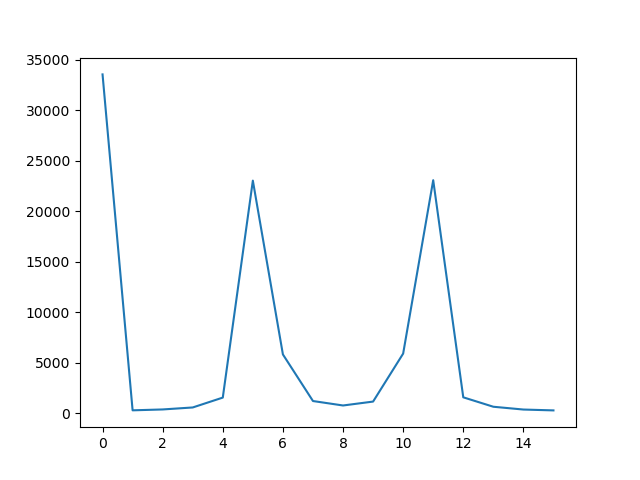
\includegraphics[width=0.6\textwidth]{./plot2.png}
      \end{center}
      \caption{result of shor execution (7 mod 30)}\label{fig:plot2}
    \end{figure}


    \begin{figure}
      \begin{center}
        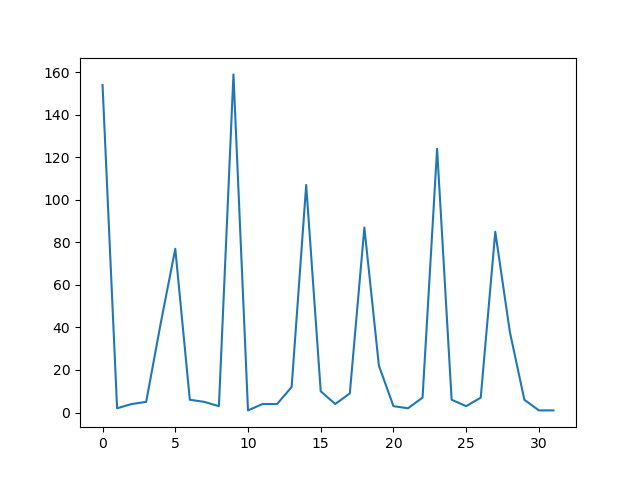
\includegraphics[width=0.6\textwidth]{./plot.png}
      \end{center}
      \caption{result of shor execution (20 mod 29)}\label{fig:plot}
    \end{figure}
    

    \begin{enumerate}
      \item What is the order $r$ of $a$ mod $N$ (here $7$ mod $30$) ?

        The order $r$ of $7$ mod $30$ is $4$.

      \item On the drawing, where are we supposed to see the values $\frac{s}{r}$ ?
        The horizontal axis is graded with integers... To what real numbers
        between 0 and 1 these correspond to ?

      \item Can you infer from the graph the value of $r$ ? Where do you see it
        on the graph ?

        Yes $r = 4$, it is presented by the period of the keys.

      \item Change a and N respectively to 20 and 29. Can you read the value $r$ ? Is it correct ?

        No I can't read the value $r$

      \item The drawing is not very precise... How to make it better ? Try it !

      \item Is it still working if you change the value of `a` and/or `N` to
        other values ? Beware not to use too large values for`N`... To get some
        inspiration, below is the list of possibilities up to 31.

        It works when the result is even.
    \end{enumerate}

\end{document}
